\documentclass[
%				draft,
xcolor=table,
PHONON=true]
{beamer}
\usepackage{color,soul}
\usepackage{xmpmulti}
%\usepackage{ppower4}
%\usepackage[table]{xcolor}% http://ctan.org/pkg/xcolor
\usepackage{helvet} %helvetica font
\usepackage{multimedia}
\usepackage{multirow}
\usepackage{booktabs}
\usepackage{tipa}
\usepackage{amsmath}
\usepackage{amsfonts}
\usepackage{amssymb}
\usepackage{pifont}
\usepackage{graphicx}
%\usepackage{setspace}
%\usepackage{nameref} 
\usepackage{pdfpages}
%\usepackage{csvsimple}
\usepackage{float}
\usepackage{pdfpages}
\usepackage[section]{placeins}
\usepackage{natbib}
	\bibliographystyle{agsm}
%\usepackage{todonotes}
%	\presetkeys{todonotes}{inline}{}
\usepackage{caption} %captions
\captionsetup{labelformat=simple} %%adds numbers to captions of figures and tables
\captionsetup{font=scriptsize,labelfont=scriptsize} %%makes it littler
%\usepackage{listings}



% THEME

%\usetheme{default}
%\usetheme{Antibes} %shows section
%\usetheme{Bergen} %sidebar
%\usetheme{Berkeley} %outline at side
%\usetheme{Berlin} %outline at top
%\usetheme{Singapore} %outline at top % faded banner at top
%\usetheme{Darmstadt} %outline at top
%\usetheme{Dresden} %outline at top
%\usetheme{Frankfurt} %outline at top
\usetheme{Ilmenau} %outline at top
%\usetheme{Madrid}

%COLOUR SCHEME

%\usecolortheme{albatross}
%\usecolortheme{beetle}
%\usecolortheme{dolphin}
%\usecolortheme{dove}
%\usecolortheme{fly}
%\usecolortheme{lily}
%\usecolortheme{orchid}
%\usecolortheme{rose}
%\usecolortheme{seagull}
%\usecolortheme{seahorse}
%\usecolortheme{whale}

%PeachPear Colour Scheme

\definecolor{PeachPearRed}{HTML}{FF3200}
\definecolor{PeachPearPeach}{HTML}{E9A17C}
\definecolor{PeachPearYellow}{HTML}{E9E4A6}
\definecolor{PeachPearTurquoise}{HTML}{1BB6AF}
\definecolor{PeachPearLightblue}{HTML}{0076BB}
\definecolor{PeachPearDarkblue}{HTML}{172869}

\setbeamercolor{background canvas}{bg=PeachPearYellow,fg=black}

\setbeamercolor{palette primary}{bg=PeachPearLightblue,fg=PeachPearPeach} %title bubble/banner
\setbeamercolor{palette secondary}{bg=PeachPearDarkblue,fg=PeachPearPeach} % ??
\setbeamercolor{palette tertiary}{bg=PeachPearDarkblue,fg=PeachPearPeach}
%
\setbeamercolor{palette quaternary}{bg=PeachPearDarkblue,fg=PeachPearPeach} %sections banner
%
\setbeamercolor{structure}{bg=PeachPearLightblue, fg=PeachPearLightblue} % itemize, enumerate, etc
%
%\setbeamercolor{section in toc}{fg=PeachPearRed} % TOC sections


%\setbeamercolor{subsection in head/foot}{bg=UBCgrey,fg=white}

%\setbeamercolor{normal text}{fg=white}
\setbeamertemplate{bibliography item}{}
%\setbeameroption{show notes on second screen=left}

% citing
\newcommand{\citeposs}[1]{\citeauthor{#1}'s (\citeyear{#1})}
\newcommand{\citefc}[1]{\citeauthor{#1} (forthcoming)}
\newcommand{\citefcp}[1]{(\citeauthor{#1} forthcoming)}
\defcitealias{PSA1868}{\textit{Public Schools Act} 1868}

% quote marks
\newcommand{\quotemarks}[1]{``#1"}
\newcommand{\quotesingle}[1]{`#1'}

%IPA
\newcommand{\ipa}[1]{\textipa{/#1/}}
\newcommand{\prel}{\ipa{l}}
\newcommand{\darkl}{[\textltilde]}
\newcommand{\goatV}{\ipa{@U}}
\newcommand{\oh}{\textipa{[@U]}}

% Lexical sets
\newcommand{\scs}{\textsc}
\newcommand{\goat}{\textsc{goat}~}
\newcommand{\goal}{\textsc{goal}~}
\newcommand{\bath}{\scs{bath}~}
\newcommand{\trap}{\scs{trap}~}
\newcommand{\foot}{\scs{foot}~}
\newcommand{\strutt}{\scs{strut}~}
\newcommand{\tilda}{$\sim$}
\newcommand{\FS}{\scs{foot}$\sim$\scs{strut}~}
\newcommand{\TB}{\scs{trap}$\sim$\scs{bath}~}
\newcommand{\palm}{\scs{palm}~}

\title{Regionality in RP: evidence from the \goat vowel}
%\subtitle{subtitle}
\author{Caitlin Halfacre}
\subject{Linguistics}
\institute{Newcastle University}
\date{\today}
%\titlegraphic{
%	
\includegraphics[width=2cm]{../img/NINElogo-transp.png}\hspace*{5cm}~
%	
\includegraphics[width=2cm]{../img/PPlogo.png} \newline \newline
%	
\includegraphics[width=2cm]{../img/UniversityCrest-transp.png}\hspace*{3cm}~
%	
\includegraphics[width=2cm]{../img/VariationLablogo-transp.png}	
%}


\begin{document}
	\frame[plain]{\titlepage}
	\begin{frame}
		\frametitle{Table of Contents}
		\tableofcontents{}
	\end{frame}
	
\section{Research Questions}

	\begin{frame}
		\frametitle{Questions}
		\begin{enumerate}
			\item In terms of pronunciation, do potential north-eastern ‘RP’ speakers behave regionally or non-regionally?
			\item What insights do these differences give us into the nature of a non-regional sociolect comprising diffuse speech communities?
		\end{enumerate}
	\end{frame}

	\begin{frame}
		\frametitle{What is RP?}
		\only{
			\begin{itemize}
				\item An accent of English
				\begin{itemize}
					\item with unusual origins \citep{Jones1917}
					\item with real speakers \citep{Fabricius2002a}
				\end{itemize}
				\item Typologically originating in the South East, lacking regional features \citep{Trudgill2002a}
				\item Change generally comes from south-eastern changes \citep{Trudgill2008}
			\end{itemize}
		}<1>
		\only{
			\begin{figure}
				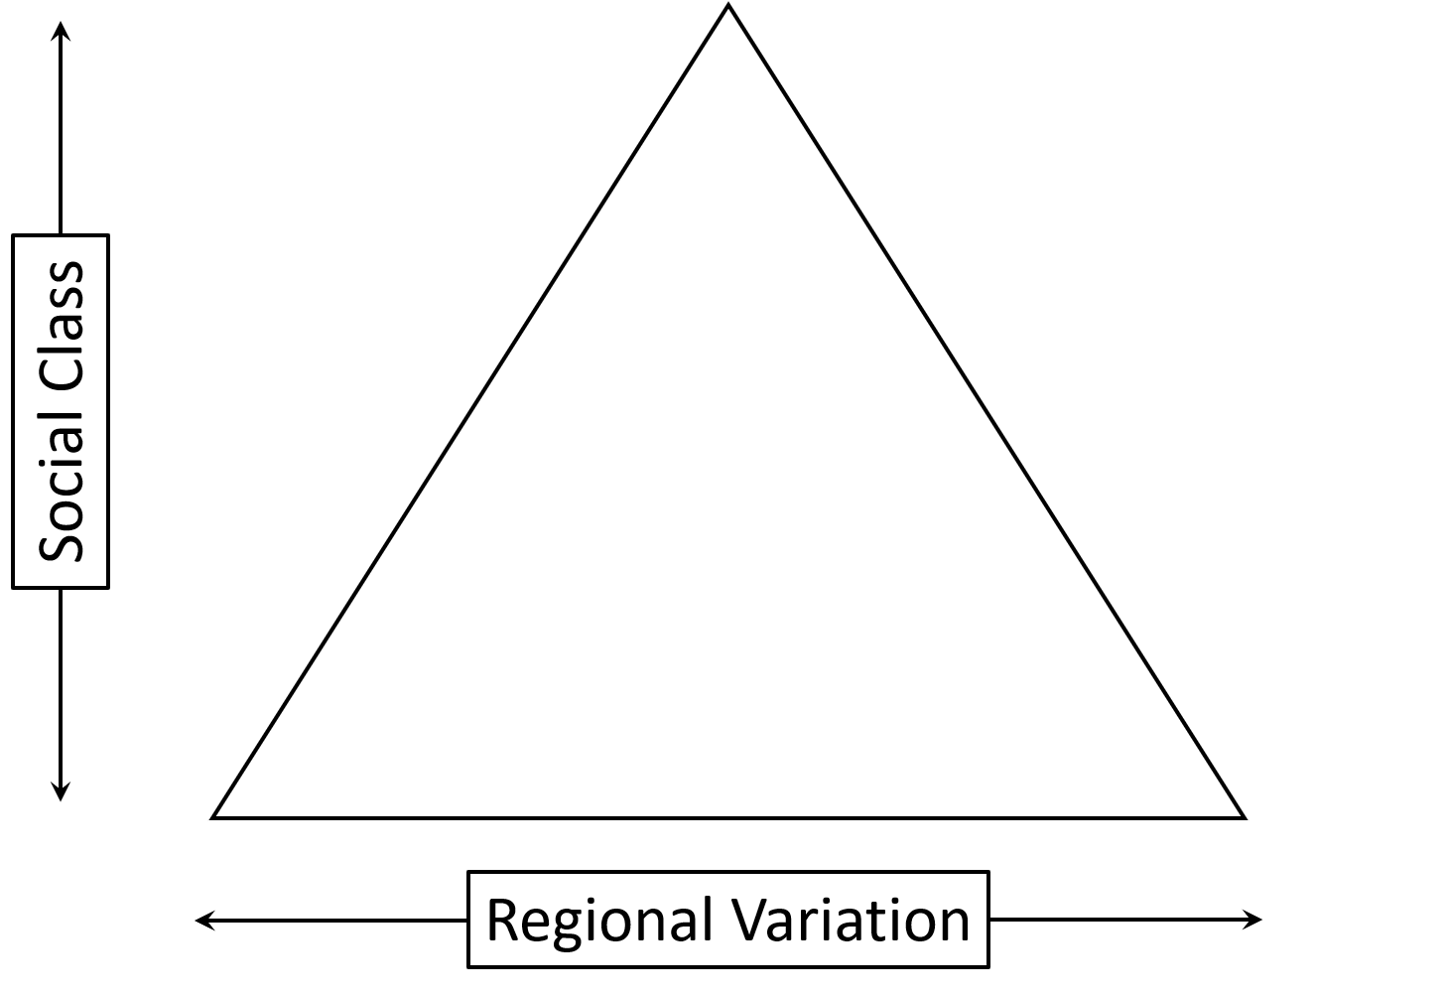
\includegraphics[scale=0.35]{../img/EnglishVariationTriangle-large-transp.png}
				\caption{(adapted from \protect\citealt{Wells1982a})}
			\end{figure}
		}<2>
	\end{frame}
%	
%	
	\begin{frame}
		\frametitle{Defining a Speaker Group}
		RP has always been tied to social class and schooling...
		\pause
		\begin{itemize}
			\item Privately Educated
			\pause
			\item Focussing on north-eastern speakers
			\pause
			\item Comparing within region and educational background
		\end{itemize}
	\end{frame}
	\begin{frame}
		\frametitle{Defining a Speaker Group}
		\framesubtitle{Locating the Variation}
		\begin{figure}
			\centering
			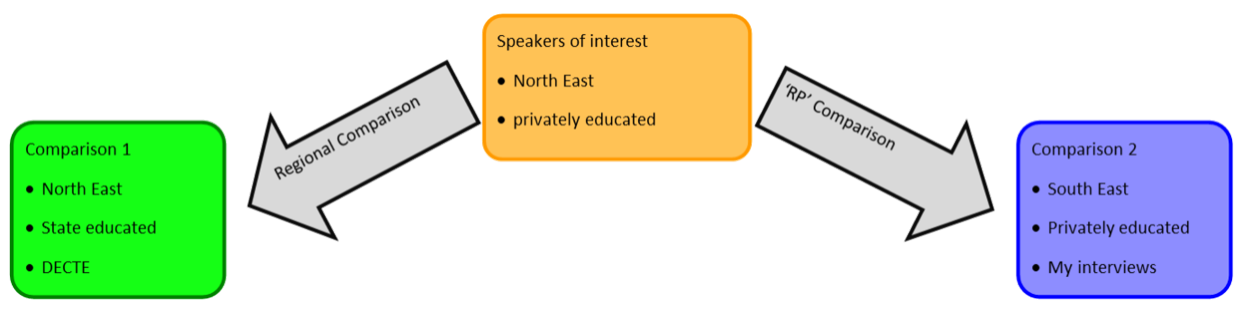
\includegraphics[scale=0.53]{../img/ComparisonMethodology-horiz.png}
		\end{figure}
	\end{frame}

\section{Why Dynamic Data?}

		\begin{frame}
		\frametitle{Previous Evidence on Regionality}
		\begin{itemize}
			\item Two vowel distinctions - \FS \& \TB
			\item 10 privately educated speakers from MA data
			\item Linear mixed effects models \citep{lme4}
		\end{itemize}
	\end{frame}
	
	\begin{frame}
		\frametitle{Previous Evidence on Regionality}
			\framesubtitle{\scs{Foot-Strut}}
			\pause
			Speakers from different regions behave similarly
			\begin{figure}
				\centering
				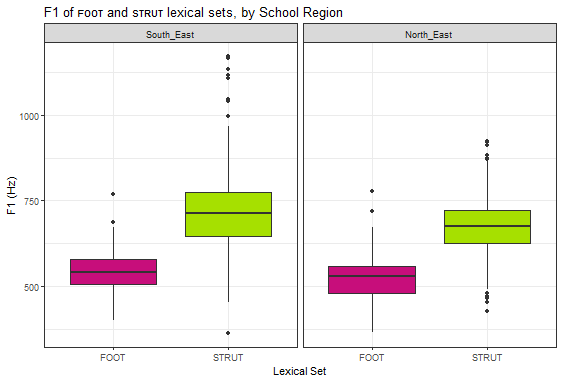
\includegraphics[width=0.7\textwidth]{../figures/UKLVC/FSF1SchR.pdf}
			\end{figure}
	\end{frame}
	
	\begin{frame}
		\frametitle{Previous Evidence on Regionality}
			\framesubtitle{\scs{Trap-Bath}}
			\pause
			Speakers behave like their region
			\begin{figure}
				\centering
				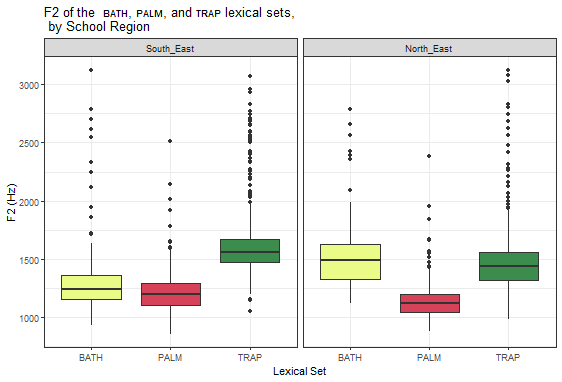
\includegraphics[width=0.8\textwidth]{../figures/UKLVC/TBF2SchR.pdf}
			\end{figure}	
	\end{frame}
	\begin{frame}
		\begin{figure}
		\only{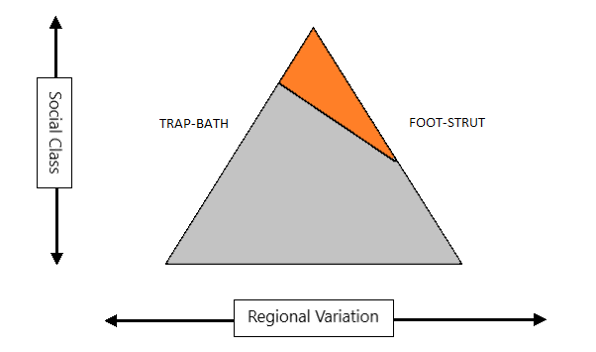
\includegraphics[scale=0.45]{../img/EnglishVariationTriangleTBFS-transp.png}}<1>
			\caption{\protect\citep{Halfacre2019}}
		\only{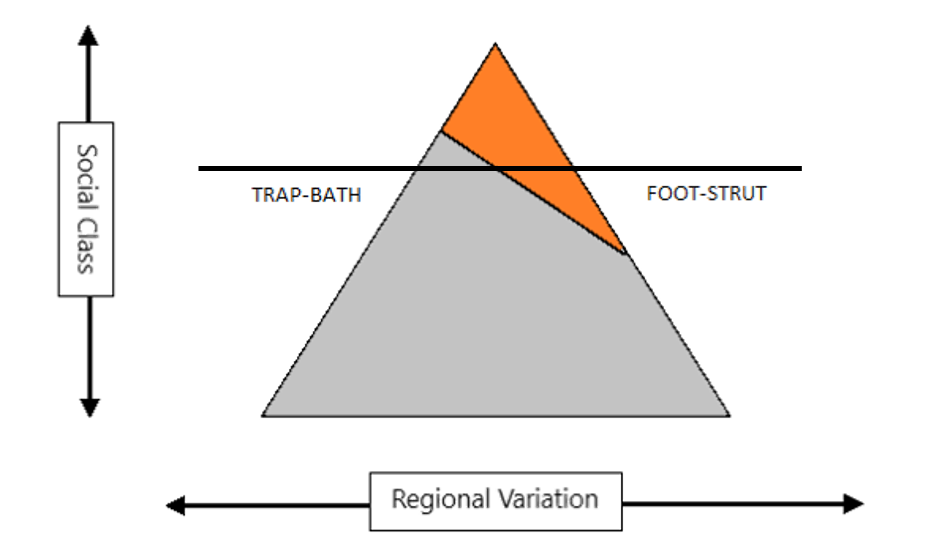
\includegraphics[scale=0.45]{../img/EnglishVariationTriangleTBFS-transp+line.png}}<2>
	\end{figure}
		
	\end{frame}

	\subsection{The \goat vowel}
	\begin{frame}
		\frametitle{\scs{Goat} Vowel Variation}
		In the North East:
		\begin{itemize}
			\item Socially stratified \citep{Watt1999}
			\begin{itemize}
				\item most common: monophthong \textipa{o:}
				\item older male speakers: traditional centring diphthong \textipa{[U@]}
				\item younger middle class speakers: national diphthong \textipa{[oU]} or \oh 
			\end{itemize}
			\item Still highly variable \citep{Warburton2021}
		\end{itemize}
		\pause
		In the South East:
		\begin{itemize}
			\item Diphthongal \oh~ since 19th century \citep{Sampson1985}
			\item Fronting occurred across the country \citep[and others]{Kerswill1996,Baranowski2017} - blocked pre lateral consonants (coda \ipa{l})
		\end{itemize}
	\end{frame}
	
	\begin{frame}
		\frametitle{\scs{Goat} Allophony}
		Originally RP generalised the fronting - no distinction between \goat and \goal - a truly non-regional feature \citep{Sampson1985}
			\begin{columns}
				\begin{column}{0.5\textwidth}
					\movie[width=\textwidth]{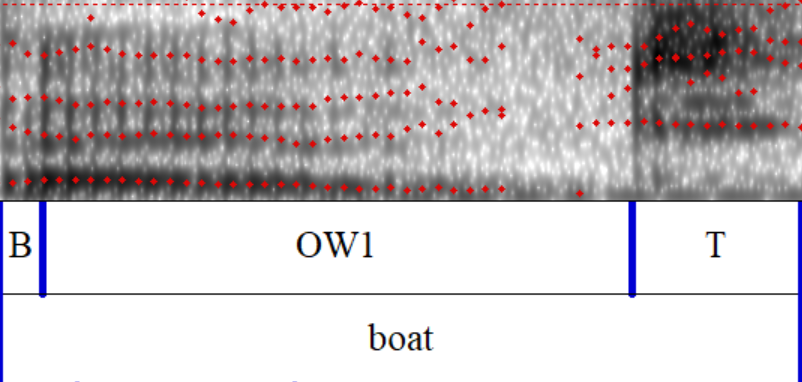
\includegraphics[width=\textwidth,height=0.5\textheight]{../img/spectro_boat.png}}{boat.mp3}
				\end{column}
				\begin{column}{0.5\textwidth}
					\movie[width=\textwidth,height=0.5\textheight]{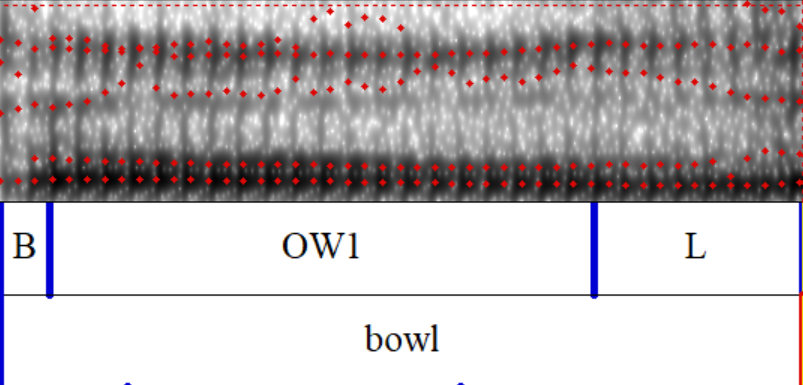
\includegraphics[width=\textwidth,height=0.5\textheight]{../img/spectro_bowl.png}}
					{bowl.mp3}
				\end{column}
			\end{columns}
	\end{frame}
	
	\begin{frame}
		\frametitle{Morphologically Complex}
		Variation in disyllabic contexts, with different morphological structures \citep{Sampson1985,Hannisdal2006}, e.g. \textit{solo, bowler}
			\begin{table}[h]
				\centering
				\begin{tabular}{lllll}
					\toprule
					& \textbf{\textit{hole}} & \textbf{\textit{hole-y}} & \textbf{\textit{holy}} & \textbf{\textit{hope}} \\
					\midrule
					\textbf{Stage 0} & \textipa{[h@Ul]} & \textipa{[h@Uli:]} & \textipa{[h@Uli:]} & \textipa{[h@Up]} \\
					\textbf{Stage 1} &	\cellcolor{PeachPearPeach}\textipa{[hOul]} & \textipa{[h@Uli:]} & \textipa{[h@Uli:]} & \textipa{[h@Up]} \\
					\textbf{Stage 2} & \cellcolor{PeachPearPeach}\textipa{[hOul]} & \cellcolor{PeachPearPeach}\textipa{[hOuli:]} & \textipa{[h@Uli:]} & \textipa{[h@Up]} \\
					\textbf{Stage 3} & \cellcolor{PeachPearPeach}\textipa{[hOul]} & \cellcolor{PeachPearPeach}\textipa{[hOuli:]} & \cellcolor{PeachPearPeach}\textipa{[hOuli:]} & \textipa{[h@Up]} \\
					\bottomrule
				\end{tabular}
				\caption{Life cycle of Phonological Processes \protect\citep{Bermudez-Otero2007a,Bermudez-Otero2012}}
				\label{lifecycle}
			\end{table}
	\end{frame}

	\begin{frame}
		\frametitle{Why Dynamic Data?}
		The \goat vowel is:
		\begin{itemize}
			\item highly variable, including monophthong or diphthong
			\item morphologically complex
		\end{itemize}
		Dynamic data analysis is fast moving into sociophonetic research \cite{Warburton2021,Cole2019}
	\end{frame}

\section{Data Collection}
	
	\begin{frame}
		\frametitle{Data Collection}
		\begin{itemize}
			\item Speakers privately educated in the North East \& South East
			\pause
			\item Sociolinguistic interviews, word lists, minimal pairs
			\pause
			\item Montreal Forced Aligner \citep{MFA} \& FAVE-extract \citep{FAVE} with script edited to extract at 10\% intervals \cite{Warburton2021}
			\item Potential problem with V/l/ segmentation - merge V/l/ in TextGrid:
			\begin{itemize}
				\item rerun extraction or
				\item extract with Praat script \& normalise in R \citep{vowels}
			\end{itemize}
		\end{itemize}
	\end{frame}
	
	


%%%%%%%%%%%%%%%%%%%%%%%%%%%%%%%%%%%%%%%%%%%%%%

%	
\section{Analysis}
	\begin{frame}
		Trajectory analysis with GAMMs \citep{itsadug,mgcv,Soskuthy2019}
			\pause
			\begin{itemize}
				\item parametric term: region or context
				\item smooths: measurement number, duration
				\item tensor product interaction: measurement number \& duration
				\item difference smooth: measurement number by region/context
				\item random smooth: trajectory
			\end{itemize}
	\end{frame}
	\begin{frame}
		\frametitle{\scs{Goat} Vowel by Region}
		\includegraphics[scale=0.35]{../figures/hope-gamm.png}
	\end{frame}
	\begin{frame}
		\frametitle{\scs{Goat} Allophony by Region (NE vs SE)}
				\begin{columns}
					\begin{column}{0.5\textwidth}
						\includegraphics[scale=0.35]{../figures/NE-gamm.png}
					\end{column}
					\begin{column}{0.5\textwidth}
						\includegraphics[scale=0.35]{../figures/SE-gamm.png}
					\end{column}
				\end{columns}
	\end{frame}
%	\begin{frame}[fragile]{Code}
%		\begin{block}{NE gamm}
%		\begin{lstlisting}[language=R]
%				NE.dur.gamm <- bam(F2 ~ lexSet_ord +
%				s(measurement.no) +
%				s(dur, bs="cr") +
%				ti(measurement.no, dur) +
%				s(measurement.no, by=lexSet_ord, bs="cr") +
%				s(measurement.no, traj, bs="fs", xt="cr", m=1, k=5),
%				data=data_NE,method="fREML", nthreads = all_cores)
%		\end{lstlisting}
%		\end{block}
%	\end{frame}

\section{Future Analysis}
	\begin{frame}
		\frametitle{Disyllabic Contexts by Region}
		\only{
			\framesubtitle{2x South-Eastern Speakers}
			\centering
			\includegraphics[scale=0.45]{../figures/di-SE-gamm-plot.pdf}
		}<1>
		\only{
			\framesubtitle{2x North-Eastern Speakers}
			\centering
			\includegraphics[scale=0.45]{../figures/di-NE-gamm-plot.pdf}
		}<2>
	\end{frame}
	\begin{frame}
		\frametitle{Further Questions}
		\begin{itemize}
			\item Is \goat allophony affected by the north-eastern \goat variation?
			\item Is the variation in disyllabic contexts affected by more fine grained social analysis: e.g. number of years in private education, parents education?
		\end{itemize}
	\end{frame}
	
%\section{References
%	\begin{frame}
%		\bibliography{bibFiles/socialClass,bibFiles/
%goatAllophony,bibFiles/lexicalPhonology,bibFiles/rRP,bibFiles/trapBath,bibFiles/soundChange,bibFiles/socialSalience,bibFiles/methodology,bibFiles/footStrut,bibFiles/socialSalience,bibFiles/tynesideEnglish}
%	\end{frame}
\end{document}